\chapter{Web extraction}
\label{chap:webextr}
Since we know the central concepts related to a webpage and its structure, we can talk about the Web extraction (WE) problem in detail. In this chapter, we will discuss modern techniques used in this area such as crawlers, wrappers and also list the complementary problems as named entity recognition and region extraction. At the end of the chapter, we will discuss related work to the thesis.\\

\textit{Web extraction} (also Web Scraping, Web harvesting) is the extraction of structured information from a webpage presented as an HTML, i.e. semi-structured text. It is important to highlight that by saying that we \textit{extract} the information from a webpage, we assume the information is located on the page and readable.


\section{Information Extraction}

The goal of Information Extraction (IE) is an automatic identification and extracting structured information from unstructured or semi-structured documents. Most of the time, in IT one processes human language. The information needed to be extracted must be explicitly specified. IE is a non-trivial task due to the complexity of natural language, and even for a limited domain implies a lot of work.\\

IE consists of several sub-tasks\cite{InfExtr}:

\begin{enumerate}
    \item \textit{Named Entity Recognition} (NER) refers to the problem of the identification and classification of predefined types of named entities, such as organizations, persons, place names, time, etc.
    \item \textit{Co-reference Resolution} (CO) requires the identification of co-referring mentions of the same entity.
    \item \textit{Relation Extraction} (RE) detects and classifies predefined relationships between identified entities.
    \item \textit{Event Extraction} (EE) refers to an identifying event in text and deriving structured information like who did what to whom, when, where, through what methods, and why. Don't confuse this sub-task of IE with the Event Extraction in the thesis, where we consider social events rather that relationships between entities in the natural language text. 
\end{enumerate}

These four sub-tasks can be considered as four well-known problems: NER refers to a segmentation and classification, RE is the association and EE is a clustering\cite{ManLect}.\\

\section{Web extraction methods}

% READ WIKI https://en.wikipedia.org/wiki/Web_scraping#Techniques\\\cite{WikiScrap}

WE can be seen as a particular case of IE where the entities are extracted not from a plain natural language text, but rather from a semi-structured HTML page. WE implies several additional sub-tasks specifically related to a webpage structure. For example, Region Extraction (RE) helps to filter web elements to focus only on relevant information. Also, since WE works with an HTML, it must entail its structure and process the tree rather than plain text. \\

World Wide Web Consortium (W3C) is an international standard organization tries to get all the players on the Web implement the same set of core principles and components. That is why all websites use relatively the same stack of technologies, and browsers seek to follow all changes and support major updates in traditional web tools.\\

Despite the fact, web developers use the same tools, HTML pages of different websites most of the time are completely different. Every site is following its design and structure, presenting the information in a different way for the particular audience of the website. That means if one method of WE works well on a specific site, it won't probably work for other sites with the same information. For that reason, WE needs to solve the problem of heterogeneity of the websites, which is the most difficult part of WE field.

\subsection{XPath and CSS}

One of the popular methods of WE from a webpage is using XPath and CSS selectors for identifying and extracting the information. The algorithm is quite simple: you look to an HTML code, find those blocks which you need to extract and compose correct XPath or CSS selectors for these web elements. After that, you can obtain the information on any webpage where such path in a DOM tree exists.  This method is the most appropriate and fast if you have one website with a big number of static pages with identical structure and design. \\

In our thesis, we use this approach as one of the steps of dataset collecting. We use Scrapy Python framework\cite{Scrapy} for identifying semantic Metadata tags and crawling the text corresponding to each tag. See example of code with Scrapy on the listing \ref{list:scrapy}.\\

\begin{lstlisting}[language=Python, caption={Example of meta tag text scrapping with Scrapy Python framework}, label={list:scrapy}, captionpos=b]
from scrapy.selector import Selector
import urllib.request as request

def get_item_types(url):
    item_types = []
    page = request.urlopen(url)
    if page.code == 200:
        html_body = page.read()
        selector = Selector(text=html_body, type="html")
        elements = selector.xpath('.//*[@itemscope]')
        for item in elements:
            item_type_text = item.xpath('@itemtype').extract()
            item_types.append(item_type_text)
    return item_types 
\end{lstlisting}

The code is self-explainable, but let's briefly discuss the main steps. Firstly, you open the webpage with urllib, that's where we send an HTTP request. If the status code is 200, meaning the positive answer from a server, we read the page. We create Scrapy Selector, and in this case, we use XPath locator. We are identifying all elements which have 'itemscope' attribute meaning we want to extract all elements which tagged with any semantic label. Then in a loop we collect all types of these semantic tag names, for example 'http://schema.org/Person', 'http://schema.org/Movie', 'http://schema.org/Event', 'http://schema.org/Place', etc. The name of the Metadata tag takes the form of URL for simplicity. \\

Obviously, the problem with this approach is no scalability, because the path in a DOM for different websites would be different. \\

\subsection{Wrappers}

\textit{Wrapper} is a general name for a program for data extraction from a webpage. In the practical application such programs are also called \textit{web crawlers} (or web spiders, web scrapers). Typically, wrappers are implemented manually by a programmer, and she needs to create a new specified wrapper for every document which has to be processed. The output of a wrapper is a structured information in some machine readable format. \\

\noindent Wrappers can be divided into three segments depending on the level of automation:
\begin{itemize}
    \item Manual wrapper: the user observers a webpage, its source code and writes down a program code to extract data (for example, using the XPath and CSS).
    \item Wrapper induction: supervised learning where extraction rules are learned from a manually labeled data records\cite{Hsu},\cite{BotUp},\cite{Stalker},\cite{Wien},\cite{Rapier}\cite{SRV}\cite{Vide}. The inductive learning process is the generalization of wrappers that are obtained from human labeled documents. 
    \item Automatic wrapper induction: unsupervised learning with the use of tree matching algorithms to find repetitive patterns on single or multiple pages\cite{Qiu},\cite{Dalvi},\cite{Diadem},\cite{Roadrunner},\cite{LiuMinData},\cite{Urest}. Automatic wrapper induction is possible because a lot of web objects follow fixed templates.
\end{itemize}

Typical usage of the wrapper as follows: a user defines set of desired attributes and indicates associated fragments of the example page. Then the program learns a wrapper for the current website. After it is done, the program uses the learned wrapper to extract new information from the same source automatically. Therefore, every step of this process may be automated to some degree. \\

Wrappers usually work well on template-based web pages, for example, a list of addresses, product catalogs, and telephone directories. There is a problem with a more unstructured page with custom design, but this kind of webpages are common on the web.

\section{Adaptive Information Extraction}

Adaptive information extraction methods can handle less structured webpages. There are three main approaches:

\begin{enumerate}
    \item First approach considers extraction task as a Classification problem which has the learning and prediction stages. For this method, one needs to have a dataset with labeled entities which needed to be extracted. 
    \item In the Sequential Labeling approach, a webpage is viewed as a sequence of words (tokens). This method can model the dependencies between target entities on the page while the classification task considering each object independently.
    \item Visual Information Extraction relies on rendering a webpage in a browser. This approach helps in extracting objects from complex web pages that may exhibit a visual pattern, but a lack of patterns in the HTML code.
\end{enumerate}

The current thesis falls into the Classification-based approach with one exception: we generate the training dataset automatically and don't imply human labeling procedure. Also, we use visual features from rendered webpage, means use ideas from Visual Information Extraction approach.\\  

More extensive surveys on different methods and works in Web Extraction field can be found in\cite{WebExtraSurveyFerrara}, \cite{Trends},\cite{WebDataSurvey}.

\section{Related problems}

\subsection{Information retrieval}

IE is closely related to Information Retrieval (IR). The task of IR is to select from a collection of textual documents a subset which is relevant to a particular query, based on key-word search and possibly augmented by the use of a thesaurus\cite{InfExtr}. A simple example of IR application is a search engine websites. You set the query, and as an output of IR algorithm, you have a list of relevant documents, ranked in descending order. In general case, there is no extracted answer from a corpus, only the documents where the answer might be. To obtain the facts or meaningful structured information from a document one needs to understand the semantic of the text on a webpage. And that's the primary goal of IE.\\

IE task considered to be harder than IR. However, IR and IE techniques are complementary and may be combined in different ways. IE often uses the IR as a filtering step, because usually, the corpus of texts is very large. IR often uses IE for the feature extraction. See figure \ref{fig:retrieval_extraction} to see the difference between IE and IR.\\

\begin{figure}[h]
\begin{center}
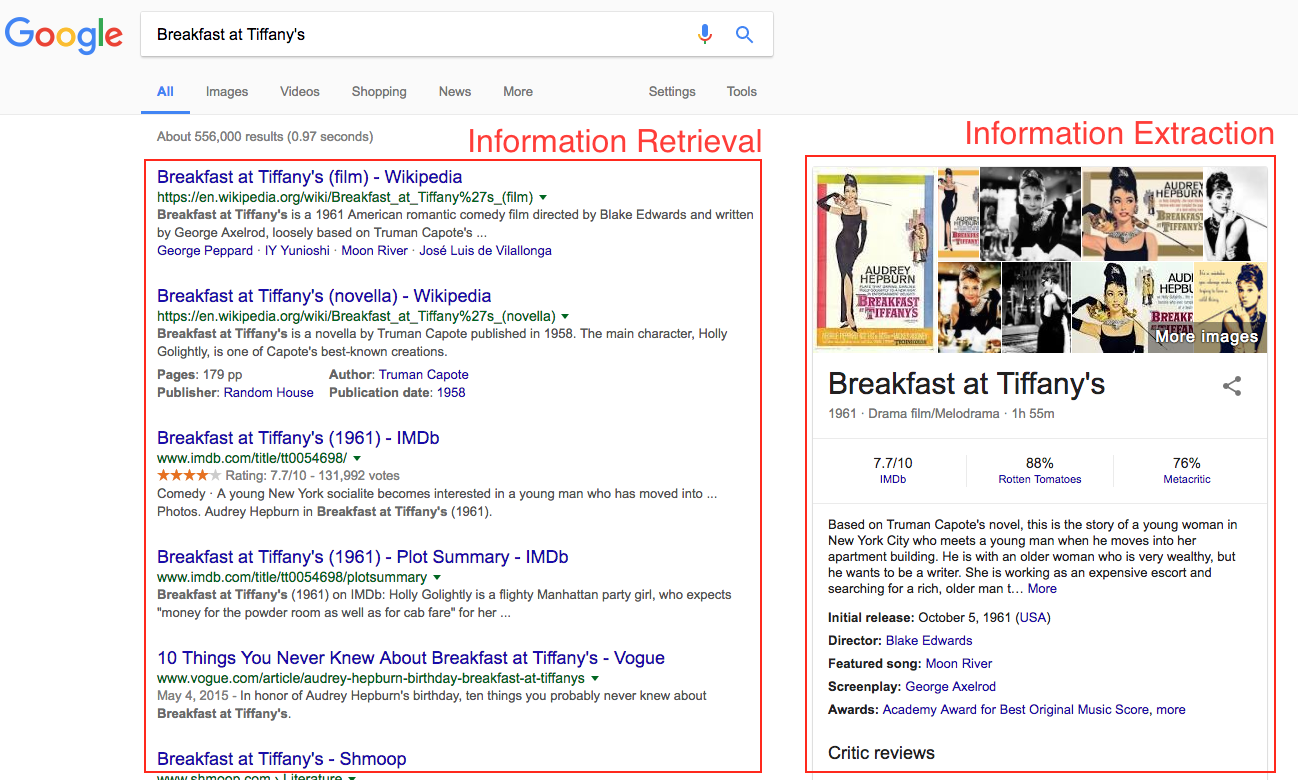
\includegraphics[width=1.0\textwidth]{figures03/retrieval_extraction}
\caption{The difference between Information Extraction and Information Retrieval}
\label{fig:retrieval_extraction}
\end{center}
\end{figure}


\subsection{Named Entity Recognition}
\textit{Named Entity Recognition (NER)} is the task of extracting entities, such as proper name (person, location, and organization), time (date and time), and numerical values (currency and percentage), from the source text, and mapping them into predefined categories, such as person, organization, location name or “none-of-the-above”\cite{MaxEntropy}. The two most important components of NER are \textit{to find} the entity and then \textit{classify} this entity. \\

NER is an essential sub-task of IE and refers to a Natural Language Processing field. \\

The uses of NER as follows\cite{ManLect}:
\begin{itemize}
    \item Named entities can be indexed, linked off, etc.
    \item Sentiment can be attributed to companies or products
    \item A lot of IE relations are associations between named entities
    \item For question answering, answers are often named entities.
\end{itemize}

There are three standard techniques to solve NER: 

\begin{enumerate}
    \item Hand-written regular expressions.
    \item Using classifiers:
    \begin{itemize}
        \item Generative: classification algorithms to classify substrings of document as “to be extracted” or not\cite{nerclass}.
        \item Discriminative: Maximum Entropy Modeling\cite{MaxEntropy}
    \end{itemize}
    \item Sequence models relies on sequential nature of natural language text:
    \begin{itemize}
        \item Hidden Markov Models\cite{HMM}
        \item Conditional Markov Models and Maximum-entropy Markov model\cite{CondModel}
        \item Conditional Random Fields\cite{ConditionalRF}
    \end{itemize}
\end{enumerate}


\subsection{Region extraction}
Web documents are getting more and more sophisticated, which complicates the task of IE. The goal of Region Extraction (RE) is filtering irrelevant information and help WE to focus only on important data records.\\

The difference between IE and RE is that IE focuses on extracting structured data about specified entity with their attributes, whereas the RE identifies the HTML block which contains this entity.\\

All region extraction methods rely on the repetitive structure of DOM tree of a webpage. The majority of region extractors are unsupervised and use tree matching, string matching, and clustering.\\

Mining Data Records (MDR) RE system\cite{LiuMinData} is based on the hypothesis that repetitive data records are usually rendered inside tables and forms. Embley et al.\cite{Embley} extract the largest unique region in a web document, supposing that this region contains relevant multiple data records. Yi et al.\cite{Noisy}, Wang and Lochovsky\cite{Wang} and Kang\cite{Kang} showed that RE has a positive impact on both efficiency and effectiveness in IE. Vision-based Page Segmentation (VIPS)\cite{Vips} built on the idea that web designers visually distinguishes the major blocks which need to be extracted. Kohlschutter\cite{Kohlschutter} utilizes the notion of text-density as a measure to identify the individual text segments of a web page.\\

The extensive list of methods on RE can be found in\cite{RegExtrSurvey}. 

\section{Web extraction as a service}

Since the task of automatic web extraction might be very useful, there are many commercial applications written for solving this task. There are both desktop and web, free and paid applications with different functionality for the extraction of specific entities. Let's consider those services which provide this functionality as an API.\\

Such applications usually offer their services on a paid basis (per number of requests) and allow to use it by any other application through HTTP requests. These APIs typically extract an only specific list of structured information. So it might be an API only for reviews or for example, only for product description in the online store. Below you will find popular web services and their main features.\\

\noindent \textbf{Diffbot's Automatic APIs}\cite{Diffbot} automatically extracts the content from supported page types: articles, discussions, images, video and products. It combines a variety of comprehensive techniques such as computer vision and machine learning. It accurately extracts clean and structured data from a webpage in JSON format without and prepossessing steps and training. One particular thing about Diffbot is that it can parse text in different languages because of extracting visual features, not only text content.\\

\noindent\textbf{ParseHub}\cite{ParseHub} parses the structured data after one example given by the user. It has an interface where the user needs to select several elements which she wants to parse, compose the rule using the visual builder and then run this scenario for the entire page. ParseHub automatically explores all elements which the user meant and parse it to JSON format. After that, this script is available as an API.\\

\noindent\textbf{Apifier}\cite{Apifier} is similar to Diffbot extracts structured information for specific topics as a product, social networks details, booking hotel websites and search engine. It presents the data in JSON format.\\

\noindent \textbf{IBM Watson}\cite{IBMAlchemy} has an Alchemy Language (part of Natural Language Understanding API) component which analyzes the data on a webpage, extracts specific entities such as people, places, and organizations with NLP methods and answer questions about these entities and its relations. IBM Watson is a huge project and includes a lot of different components related to natural language understanding, speech, and visual recognition.\\  

\noindent\textbf{Other services}. There are dozens of web services which offer article content extraction, especially the name and description. Also there several interesting services which extract entities from an unstructured plain text: Ambiverse Natural Language Understanding\cite{Ambiverse}, Google Cloud Natural Language\cite{GoogNLP}, Calais by Reuters\cite{calais}. Entities are identified by types such as a person, location, organization, product, etc.

\section{Related work}

There are not much work about social event extraction. The closest work is made by Google Research\cite{GoogEvent} which similarly to us used semantic markup together with a large human-labelled dataset. Petrovski et al.\cite{Petrovski} use Schema.org annotations for product ads to learn regular expressions. Gentile et al.\cite{Gentile} work on dictionary-based wrapper induction methods that learn XPaths using linked data. Becker\cite{becker} was identifying
and characterizing events in social media channels. Gogar et al.\cite{Gogar2016}
presented an automatic method based on the deep neural network to extract information from e-commerce websites.

\section*{Conclusion of the chapter}
In this chapter, we discussed theoretical background in IE and WE fields, reviewed the main works and presented related problems as region extraction, named entity recognition and information retrieval. Also we listed several commercial IE web services and briefly explained how they work.